% no answer key
% \documentclass[letterpaper]{exam}

% answer key
\documentclass[letterpaper, landscape]{exam}
\usepackage{2in1, lscape} 
\printanswers{}

\usepackage{units} 
\usepackage{xfrac} 
\usepackage[fleqn]{amsmath}
\usepackage{cancel}
\usepackage{float}
\usepackage{mdwlist}
\usepackage{booktabs}
\usepackage{cancel}
\usepackage{polynom}
\usepackage{caption}
\usepackage{fullpage}
\usepackage{comment}
\usepackage{enumerate}
\usepackage{graphicx}
\usepackage{parskip}
\usepackage[group-separator={,}]{siunitx}

\everymath{\displaystyle}

\title{Statistics \\ Chapters 10 and 12}
\date{\today}
\author{}

\begin{document}

  \maketitle

  \ifprintanswers{}
  \else
    \section{Homework}
    \begin{itemize*}
      \item Chapter 10: 31, 33--38, 40--44, 47--53
      \item Chapter 12: 27--32, 34--36, 38--40, 44--46, 49, 51, 54--56
    \end{itemize*}
  \fi

  \ifprintanswers{}
  \section{Chapter 10} % (fold)
  
    \begin{description}

      \item[31] 
        \begin{enumerate}[(a)]
          \item If you are recording the sequence, the order matters.  If 1 is a
            make and 0 a miss, the sample space would be 
            
            \{ 0000, 0001, 0010, 0011, 0100, 0101, 0110, 0111, 1000, 1001, 1010,
               1011, 1100, 1101, 1110, 1111 \}

          \item If you don't care about the order, the sample space is just the
            number of shots made, or {0, 1, 2, 3, 4 }

        \end{enumerate}

      % \item[32]
      %   \begin{enumerate}[(a)]
      %     \item The probabilities are all less than 1 and add up to 1, so they
      %       satisfy the rules of probability.  They aren't the correct
      %       probabilities for an actual die, however.

      %     \item The probabilities are all less than 1 and add up to 1, so they
      %       satisfy the rules of probability.  They aren't the correct
      %       probabilities for an actual card deck, however.

      %     \item These probabilities don't add up to exactly 1, so they don't
      %       satisfy the rules of probability.  
      %   \end{enumerate}

      \item[33]
        \begin{enumerate}[(a)]
          \item This is the only probability not provided, so it is:
            \[
              1 - 0.13 - 0.29 - 0.30 = \boxed{ 0.28 }
            \]

          \item This is everybody except the people that didn't complete high
            school:
            \[
              1 - 0.13 = \boxed{ 0.87 }
            \]
        \end{enumerate}

      \item[34]
        \begin{enumerate}[(a)]
          \item $\frac{\num{ 4 176 000 }}{\num{ 9 094 000 }} \approx \boxed{ 0.46 }$
          \item $1 - 0.46 \approx \boxed{ 0.54 }$
        \end{enumerate}

      \newpage 

      \item[35]
        \begin{enumerate}[(a)]
          \item The probabilities are disjunct and add up to 1.
          \item $1 - 0.59 = \boxed{ 0.41 }$
          \item $0.26 + 0.09 + 0.03 = \boxed{ 0.38 }$
        \end{enumerate}

      \item[36]
        \begin{enumerate}[(a)]

          \item The probabilities listed add up to 0.9, so the probability of
            any other color is \boxed{ 0.1 }.

          \item The probability of silver or white is: $0.19 + 0.18 = 0.37$. The
            probability of any other color is: $1 - 0.37 = \boxed{ 0.63 }$.

        \end{enumerate}

      \item[37]
        \begin{enumerate}[(a)]
          \item $\sfrac{3}{7} \approx \boxed{ 0.43 } $
          \item $\sfrac{2}{7} \approx \boxed{ 0.29 } $
          \item $\sfrac{5}{7} \approx \boxed{ 0.71 } $
        \end{enumerate}

      \item[38]
        For an unloaded die, the probability for any face coming up is:
        \[
          \frac{1}{6} \approx 0.17
        \]

        The probability of something other than a 1 or a 6 is:
        \[
          \frac{4}{6} \approx 0.6667
        \]

        Since this probability is unaffected, the probability of getting a 1 for
        the loaded die is:
        \[
          1 - 0.2 - 0.6667 \approx 0.1333
        \]

        The probabilities for all the numbers are:
        \begin{itemize*}
          \item 1: \boxed{ 0.1333 }
          \item 2, 3, 4, 5: \boxed{ 0.1667 }
          \item 6: \boxed{ 0.2 }
        \end{itemize*}

      % \item[39]
      %   With 48 men and 42 women, there are 90 people at the party. 42 of the 90
      %   are women, so the chance of a woman winning the prize is:
      %   \[
      %     42 / 90 \approx \boxed{ 0.4667 }
      %   \]

      \newpage

      \item[40]
        \begin{enumerate}[(a)]
          \item They add up to 1, so they are a legitimate set of probabilities.

          \item The sum of the Hispanic probabilities is $\boxed{ 0.149 }$

          \item $1 - 0.674 = \boxed{ 0.326 }$
        \end{enumerate}

      \item[41]
        \begin{enumerate}[(a)]
          \item The probabilities add up to 1.

          \item $\boxed{ 0.04 }$

          \item $0.11 + 0.04 + 0.03 = \boxed{ 0.18 }$

          \item $0.04 + 0.09 + 0.13 + 0.16 = \boxed{ 0.42 }$

        \end{enumerate}

      \item[42]
        \begin{enumerate}[(a)]
          \item Everything in either the ``19 years old'' column or the ``Own Place'' row or both.

          \item The value for 19 year olds who live in their own place would be
            counted twice since you can be both 19 years old and living in your own place.

        \end{enumerate}  

      \item[43]
        \begin{enumerate}[(a)]
          \item $0.11 + 0.13 + 0.03 + 0.11 + 0.16 + 0.02 = \boxed{ 0.56 }$

          \item The probability of living with parents is:
            \[
              0.11 + 0.13 + 0.11 + 0.11 = 0.46
            \]

            The probability of not living with parents is:
            \[
              1 - 0.46 = \boxed{ 0.54 }
            \]
        \end{enumerate}  

      \item[44]
        \begin{enumerate}[(a)]
          \item A word is either right or wrong, (it can't be half right) so the
            variable is \fbox{ discrete }.

          \item $P(X \geq 1) = 0.2 + 0.3 + 0.3 + 0.1 = \boxed{ 0.9 }$

          \item $P(X \leq 2)$ is the probability that there were 2 or fewer errors.
            \begin{align*}
              P(X < 2) & = 0.1 + 0.2 \\
                       & = \boxed{ 0.3 } \\
              \\
              P(X \leq 2) & = 0.1 + 0.2 + 0.3 \\
                          & = \boxed{ 0.6 } \\
            \end{align*}
        \end{enumerate}  

      % \item[45]
      %   \begin{enumerate}[(a)]
      %     \item Each choice has a $1/9 \approx \boxed{ 0.11 }$ chance of being selected.
      %     \item $P(X \geq 6) = 4/9 \approx \boxed{ 0.44 }$
      %   \end{enumerate}  

      \item[47]
        \begin{enumerate}[(a)]
          \item GGG, GGB, GBG, GBB, BGG, BGB, BBG, BBB
          \item $P(X = 2) = \sfrac{3}{8} = \boxed{ 0.375 }$

          \item
            \begin{tabular}[H]{lrrrr}
              \toprule
              Value of X  & 0     & 1     & 2     & 3 \\
              \midrule
              Probability & 0.125 & 0.375 & 0.375 & 0.125 \\
              \bottomrule
            \end{tabular}
        \end{enumerate}  

      \item[48]
        All of the numbers between 1 and 12 have an equal probability of
        approximately $\boxed{ 0.083 }$

      \item[49]
        \begin{enumerate}[(a)]
          \item \fbox{ Continuous }, since any number may be selected.

          \item Since the area is 1 and the base is 2, the height is $\boxed{ 0.5 }$.

          \item $P(X \leq 1) = \boxed{ 0.5 }$

        \end{enumerate}  

      \item[50]
        \begin{enumerate}[(a)]
          \item $P(0.5 < Y \leq 1.3) = 0.5 \cdot 1.3 - 0.5 \cdot 0.5 = \boxed{ 0.4 }$
          \item $P(Y \geq 0.8) = 1 - 0.8 \cdot 0.5= \boxed{ 0.6 }$
        \end{enumerate}  

      \item[51]
        \begin{enumerate}[(a)]
          \item Convert 0.52 and 0.60 to z-scores:
            \begin{align*}
              z_1 & = \frac{0.52 - 0.56}{0.019} \approx -2.1 \\
              z_2 & = \frac{0.60 - 0.56}{0.019} \approx 2.1 \\
            \end{align*}

            Use table A to find the fraction below each of these:
            \begin{align*}
              p_1 &\approx 0.0176 \\
              p_2 &\approx 0.9824 \\
            \end{align*}

            Subtract:
            \[
              P(0.52 \leq V \leq 0.60) \approx 0.9824 - 0.0174 = \boxed{ 0.9647 }
            \]

          \item Convert 0.72 to a z-score:
            \begin{align*}
              z & = \frac{0.72 - 0.56}{0.019} \\
                & \approx 8.4 \\
            \end{align*}

            Table A doesn't go this high, so $P(V \geq 0.720) \approx 0$
        \end{enumerate}  

      \item[52]
        \begin{enumerate}[(a)]
          \item Convert to z-scores:
            \begin{align*}
              z_1 & = \frac{8.9 - 9}{0.075} \approx -1.33 \\
              z_2 & = \frac{9.1 - 9}{0.075} \approx 1.33 \\
            \end{align*}

            Use table A to find the fraction below each of these:
            \begin{align*}
              p_1 &\approx 0.0912 \\
              p_2 &\approx 0.9088 \\
            \end{align*}

            Subtract:
            \[
              P(8.9 \leq \bar{X} \leq 9.1) \approx 0.9088 - 0.0912 = \boxed{ 0.8176 }
            \]
          \end{enumerate}

        \item[53]
          \begin{enumerate}[(a)]
            \item $1/10,000 = \boxed{ 0.0001 }$

            \item There are 4 different choices for the first digit, 3 choices
              for the second digit, once you've selected the first digit, 2
              choices for the third digit once you've selected the first 2, and
              only one choice for the remaining digit. The total number of ways
              to rearrange the digits is:
              \[
                4 \times 3 \times 2 = 24
              \]

              The chance of those digits coming up in any order is:
              \[
                24 / 10,000 = \boxed{ 0.0024 }
              \]
          \end{enumerate}

  \end{description}

  \section{Chapter 12} % (fold)
  
  \begin{description}

    \item[27] 
      The probability of each bet losing is 0.75. Since the bets are
      independent, the probability of all 8 losing is
      \[
        p_{fail} = 0.75^8 \approx \boxed{ 0.1001 }
      \]

    \item[28]
      There is a 92.8\% chance of a person not being a universal donor. The
      probability one of the 10 being a universal donor is:
      \[
        p = 1 - 0.928^{10} \approx \boxed{ 0.5263 }
      \]

    \item[29]
      \begin{enumerate}[(a)]
        \item 
          \[
            \frac{9}{20} \cdot \frac{1}{20} \cdot \frac{1}{20} 
              \approx \boxed{ 0.0011 }
          \]

        \item
            The probability that wheel 1 and exactly one of the other two
            wheels both show a cherry is:
            \[
              \frac{9}{20} \cdot \frac{1}{20} \cdot \frac{19}{20} 
                \approx \boxed{ 0.0214 }
            \]

            The probability that wheel 1 doesn't show a cherry and wheels 2 and 3 
            do is:
            \[
              \frac{11}{20} \cdot \frac{1}{20} \cdot \frac{1}{20} 
                \approx \boxed{ 0.0014 }
            \]

          \item
            Since the events are disjunct, you can add them:
            \[
              p \approx 2 \cdot 0.0214 + 0.0014 \approx \boxed{ 0.0441 } 
            \]
      \end{enumerate}

    \item[30]
      \begin{enumerate}[(a)]
        \item 
          \[
            p_{up} = 0.65^3 \approx \boxed{ 0.2746 }
          \]

        \item 
          The probability it goes down for 3 years in a row is:
          \[
            p_{down} = 0.35^3 \approx 0.0429
          \]

          The probability of 3 consecutive years of either loss or gain is:
          \[
            p \approx 0.2746 + 0.0429 = \boxed{ 0.3175 }
          \]

      \end{enumerate}

    \item[31]
      \begin{enumerate}[(a)]
        \item The probability that neither one admits him is:
          \[
            p_{reject} = 0.6 \cdot 0.5 = \boxed{ 0.3 }
          \]

          Another way to figure this out is to find the probability that he
          gets in to either one and then subtract this from 1:
          \begin{align*}
            p_{accept} & = 0.4 + 0.5 - 0.4 \cdot 0.5 = 0.7 \\
            p_{reject} & = 1 - p_{accept} \\
                       & = 1 - 0.7 \\
                       & = 0.3
          \end{align*}

        \item
          This is the probability he gets into Stanford minus the probability
          he gets into both:
          \[
            p = 0.5 - 0.5 \cdot 0.4 = \boxed{ 0.3 }
          \]
          
        \item 
          \begin{align*}
            P( \text{Stanford } | \text{ Princeton } ) & = \frac{ P(\text{ Stanford and Princeton }) }{ P(\text{ Princeton }) } \\
                                                       & = \frac{0.2}{0.4} \\
                                                       & = 0.5 \\
          \end{align*}

          Since $P(\text{Stanford } | \text{ Princeton}) = P(\text{Stanford})$, the events are \fbox{ independent }.

      \end{enumerate}

    \item[32]
      \begin{enumerate*}
        \item 1\% of the cases are infections with failed surgeries
        \item 2\% of the cases are infections with successful surgeries
        \item 14\% of the cases are failed surgeries with or without infection
      \end{enumerate*}

      The probability of a bad outcome is covered by cases 2 and 3, since case 1
      is included in case 3. If the surgery failed, the result was bad, and
      getting an infection only makes a bad result worse.
      
      Since the probability of a bad outcome is 16\%, the probability of a
      successful surgery without infection is \fbox{ 84\% }.

      It would be nice if the surgeon figured this out for you so you didn't
      have to do math while worrying about your knee.

    % \item[33] Since the various ways to reach outcome D are mutually
    %   exclusive, we can add them to get the probability of D:
    %   \[
    %     p_{D} = 0.1 + 0.1 + 0.2 = \boxed{ 0.4 }
    %   \]

    \item[34]
      The probability of studying some language is $1 - 0.59 = 0.41$
      \[
        P(\text{Spanish } | \text{ Language}) = \frac{0.26}{0.41} 
          \approx \boxed{ 0.63 }
      \]

    \item[35]
      \begin{enumerate}[(a)]
        \item 
          \[
            p = 0.215 + 0.1 + 0.006 = \boxed{ 0.321 }
          \]

        \item
          \[
            p = \frac{0.1 + 0.006}{0.321} \approx \boxed{ 0.3302 }
          \]
      \end{enumerate}

    \item[36]
      \begin{enumerate}[(a)]
        \item 
          \begin{align*}
            P(\text{mushroom } | \text{ thick}) & = \frac{2}{3} \\
            P(\text{mushroom})                  & = \frac{1}{2} \\
          \end{align*}

          Since $P(\text{mushroom } | \text{ thick}) \ne P(\text{mushroom})$,
          the events are \fbox{ not independent }.
          
        \item 
          \begin{align*}
            P(\text{mushroom } | \text{ thick}) & = \frac{1}{2} \\
            P(\text{mushroom})                  & = \frac{1}{2} \\
          \end{align*}
          
          Since $P(\text{mushroom } | \text{ thick}) = P(\text{mushroom})$,
          the events are \fbox{ independent }.
      \end{enumerate}

    % \item[37]
    %   The part of the square where $y < \sfrac{1}{2}$ is the bottom half of the
    %   square.

    %   The part of the square where $y > x$ is the part of the square above the
    %   diagonal.

    %   The intersection of these two sections is one fourth of the part of the
    %   square above the diagonal, so the probability is $\boxed{ 0.25 }$.

    \item[38]
      \begin{enumerate}[(a)]
        \item One of the three boy-containing pairs is two boys, so the
          probability is:
          \[
            p = \frac{1}{3} \approx \boxed{ 0.3333 }
          \]

        \item If the first child is a boy, then her two kids are either BB or
          BG and the probability of BB is \fbox{ 0.5 }.
      \end{enumerate}

    \item[39]
      \begin{enumerate}[(a)]
        \item 
          \[
            P(\text{woman}) = \frac{1481}{2506} \approx \boxed{ 0.59 }
          \]

        \item
          Since 32 out of the 59 doctoral degrees are women:
          \[
            P( \text{woman } | \text { doctorate} ) = \frac{32}{59} 
              \approx \boxed{ 0.5424 }
          \]

          alternate approach:
          \begin{align*}
            P( \text{doctorate} )                   & = \frac{59}{2506} \approx 0.0235 \\
            P( \text{woman and doctorate} )         & = \frac{32}{2506} \approx 0.0128 \\
            P( \text{woman } | \text { doctorate} ) & = \frac{0.0128}{0.0235}
              \approx 0.5424 \\
          \end{align*}

        \item They aren't independent because 
          \[
            P(\text {woman}) \neq P( \text{woman } | \text { doctorate} )
          \]

      \end{enumerate}

    \item[40]
      \begin{enumerate}[(a)]
        \item 
          \[
            P(\text{man}) = \frac{1025}{2506} \approx \boxed{ 0.4090 }
          \]

        \item

          Since 693 of the male degree recipients got bachelor's degrees:
          \[
            P( \text{bachelors } | \text { man} ) = \frac{693}{1025} 
              \approx \boxed{ 0.6761 } 
          \]

          alternate approach:
          \begin{align*}
            P( \text{man and bachelors} )         & = \frac{693}{2506} \approx 0.2765 \\
            P( \text{bachelors } | \text { man} ) & = \frac{0.2765}{0.4090}
              \approx 0.6761 \\
          \end{align*}
        \item Using the probability rule:
          \begin{align*}
            P( & \text{bachelors and man}) = 
              P( \text{bachelors } | \text { man} ) \cdot P( \text{man} ) \\
              & \approx 0.6761 \cdot 0.4090  \\
              & \approx \boxed{ 0.2765 }  \\
          \end{align*}

          From the counts:
          \[
            P( \text{bachelors and man}) \approx \frac{693}{2506} \approx 0.2765 
          \]

      \end{enumerate}

    % \item[41]
    %   \begin{enumerate}[(a)]
    %     \item 209 out of 871 seedlings were damaged:
    %       \[
    %         \frac{209}{871} \approx \boxed{ 0.2400 }
    %       \]


    %     \item
    %       \begin{tabular}[H]{lr}
    %         \toprule
    %         Cover      & Probability of Damage \\
    %         \midrule
    %         none       & 0.28 \\
    %         <1/3       & 0.32 \\
    %         1/3 to 2/3 & 0.20 \\
    %         >2/3       & 0.14 \\
    %         \bottomrule
    %       \end{tabular}

    %     \item In general, more cover means less damage, so they aren't independent.

    %   \end{enumerate}

    \item[44]
      The probability of at least one is the sum of the probabilities for the individual
      jobs minus the overlaps:
        \[
          p = 0.6 + 0.4 + 0.2 - 0.1 - 0.05 - 0.05 = \boxed{ 1.0 }
        \]

        Julie is very confident.

    \item[45]
      Since there is 0 probability of her getting all three offers, this is just the
      probability of her getting the other two offers, or \fbox{ 0.1 }.

    \item[46]
      \begin{align*}
        P(B|C) &= \frac{0.05}{0.2} = \boxed{ 0.25 } \\
        P(C|B) &= \frac{0.05}{0.4} = \boxed{ 0.125 } \\
      \end{align*}

    % \item[47]
    %   \begin{enumerate}[(a)]
    %     \item There are 6 doubles outcomes, so the probability is
    %       \[
    %         p = \frac{6}{36} = \boxed{ \frac{1}{6} }
    %       \]

    %     \item 
    %       \[
    %         p = \frac{5}{6} \cdot \frac{1}{6} = \boxed{ \frac{5}{6^2} }
    %       \]

    %     \item 
    %       \[
    %         p = \frac{5}{6} \cdot \frac{5}{6} \cdot \frac{1}{6} 
    %           = \boxed{ \frac{5^2}{6^3} }
    %       \]

    %     \item
    %       \[
    %         p = \frac{5^{k - 1}}{6^k}
    %       \]

    %   \end{enumerate}

    % \item[48]
    %   \begin{figure}[H]
    %     \centering
    %     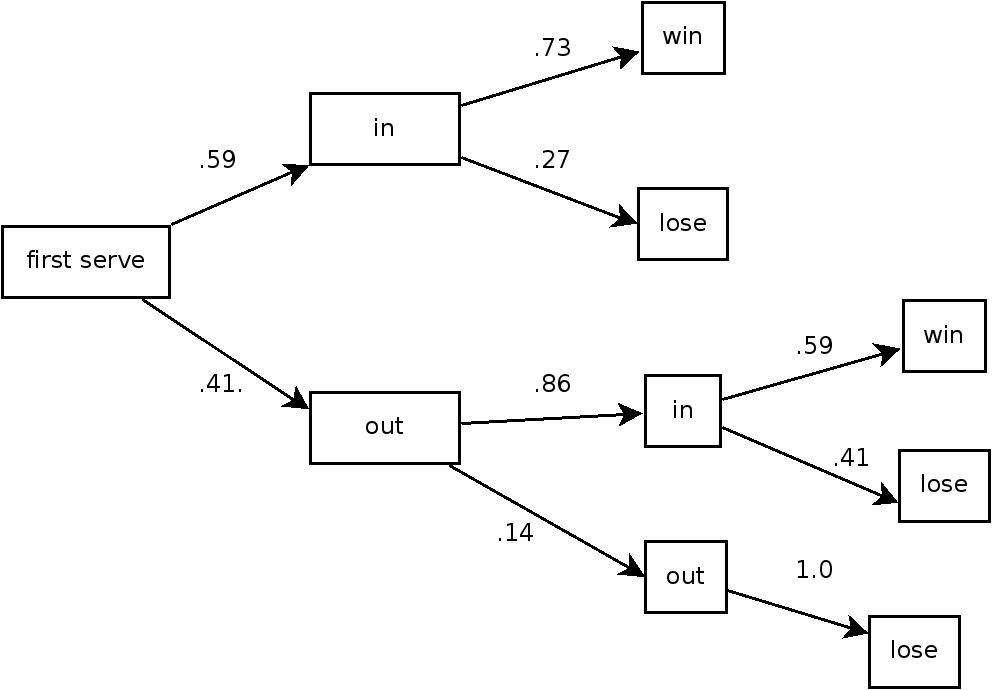
\includegraphics[scale = 0.2]{ex48.jpg}
    %     \caption{Exercise 48}
    %   \end{figure}

    %   The chance of winning by getting the first serve in is:
    %   \[
    %     p_{1st} = 0.59 \cdot 0.73 = 0.4307
    %   \]
    %   The chance of winning by getting the second serve in is:
    %   \[
    %     p_{2nd} = 0.41 \cdot 0.86 \cdot 0.59 = 0.2080
    %   \]

    %   Since these two events are disjoint, the probability of the serving player
    %   winning the point is
    %   \[
    %     p_{win} = 0.4307 + 0.2080 \approx \boxed{ 0.6387 }
    %   \]

    \item[49]
      % \begin{figure}[H]
      %   \centering
      %   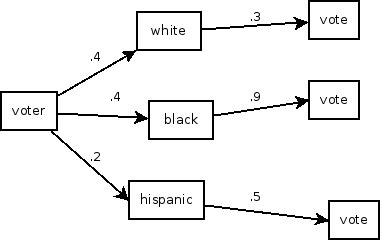
\includegraphics[scale = 0.4]{ex49.jpg}
      %   \caption{Exercise 49}
      % \end{figure}

      \begin{align*}
        p_{white} = 0.4 \cdot 0.3 = 0.12 \\
        p_{black} = 0.4 \cdot 0.9 = 0.36 \\
        p_{hispanic} = 0.2 \cdot 0.5 = 0.1 \\
        \\
        p_{total} = 0.12 + 0.36 + 0.1 = \boxed{ 0.58 } \\
      \end{align*}

    % \item[50]
    %   Given that the server won the point, what was the probability that the first
    %   serve was in?

    %   \begin{align*}
    %     P(\text{in } | \text{ won}) & = \frac{P(\text{in and won})}{P(\text{won})} \\
    %                 & \approx \frac{0.4307}{0.6387} \\
    %                 & \approx \boxed{ 0.6743 } \\
    %   \end{align*}

    \item[51]
      Given that the vote was won, what was the probability that the voter was black?

      \begin{align*}
        P(\text{black } | \text{ won}) & = \frac{P(\text{black and won})}{P(\text{won})} \\
                       & \approx \frac{0.36}{0.58} \\
                       & \approx \boxed{ 0.6207 } \\
      \end{align*}

    \item[54]
      \begin{enumerate}[(a)]
        \item A, B and AB

        \item
          The four combinations you might get are AA, AB, BA, and BB\@. Since there are 
          two ways to get different alleles, this is twice as likely and the probabilities
          are:
          \begin{align*}
            P(A)  & = P(B) = 0.25 \\
            P(AB) & = 0.5 \\
          \end{align*}
      \end{enumerate}

    \item[55]
      \begin{enumerate}[(a)]
        \item B and O

        \item
          The four combinations you might get are BB, BO, OB, and OO\@. There is
          only one way two way to end up with type O and three ways to end up
          with B. The probabilities are
          \begin{align*}
            P(B) & = 0.75 \\
            P(O) & = 0.25 \\
          \end{align*}
      \end{enumerate}

    \item[56]
      \begin{enumerate}[(a)]
        \item 
          With these parents, the possible blood types for the children are: 
          
          A (0.5), AB (0.25), B (0.25)

          The probability of 2 As is 
          \[
            0.5^2 = \boxed{ 0.25 }
          \]

        \item 
          \begin{align*}
            P(same) & = 0.5^2 + 0.25^2 + 0.25^2 \\
                    & = \boxed{ 0.375 }
          \end{align*}
      \end{enumerate}
  \end{description}
  \else
    \vspace{10 cm}
    \begin{quote}
      \begin{em}
        Is a democracy, such as we know it, the last improvement possible in
        government? Is it not possible to take a step further towards
        recognizing and organizing the rights of man? There will never be a
        really free and enlightened State until the State comes to recognize the
        individual as a higher and independent power, from which all its own
        power and authority are derived, and treats him accordingly. 
      \end{em}
    \end{quote}
    \hspace{1 cm} --Henry David Thoreau
  \fi

\end{document}

